\documentclass[11pt]{cernrep}
\usepackage{graphicx,epsfig}
\bibliographystyle{lesHouches}
\begin{document}


\title{Supersymmetric Technicolour in Warped Spaces and Crooked
Places}

\author{B. Nobalma$^1$, N. Schlamoky$^2$, K. Weasel$^2$}
\institute{$^1$LAPTH, 9 Chemin de Bellevue, B.P. 110,
Annecy-le-Vieux 74951, France
\\$^2$Tate Gallery of Fundamental
Research,  Trunka}

\maketitle

\begin{abstract}
We examine resonant techni-sleptons production at the LHC with
gravitinos in the final state. We investigate two cases: (i) where
the slepton undergoes gauge decay into neutralino and a lepton,
followed by the neutralino decay into a photon and a gravitino,
and (ii) direct decays of a slepton into a lepton and a gravitino.
We show how to accurately reconstruct both the slepton and
neutralino masses in the first case, and the slepton mass in the
second case for 300 fb$^{-1}$ of integrated luminosity at the LHC.
\end{abstract}

\section{INTRODUCTION}
This letter is devoted to the study of the signals at the Large Hadron
Collider (LHC) due to a supersymmetric generalisation of the Standard
Model (SM) which (a) violates $R$-parity, and (b) has an ultra-light
gravitino in its spectrum. The anomalous events in the CDF experiment
in the production rate of lepton-photon-${\not\!\!E}_{T}$ in $p{\bar p}$ collisions
were explained~\cite{Belanger:2001fz,Binoth:2005ff,Huston:2011ny}
in the framework of a
$R$-parity violating supersymmetric model with dominant
$L$-violating $\lambda'_{211}$ coupling,
and an ultra-light gravitino of mass $\sim10^{-3}$ eV.

The resonant production of a smuon via the $R$-violating coupling,
its decay into neutralino and a muon and, finally, the decay of the
neutralino into a gravitino and a photon
leads to the $\mu \gamma {\not\!\!E}_{T}$ final state studied in the CDF experiment.
The range of smuon and neutralino masses rel<evant to the explanation of
these
anomalous observations of the the CDF experiment is such that most of
this range will be explored at the Run II of the Tevatron.
In the event
that this signal is not seen at Run II it will rule out the model at
the lower end of the neutralino and smuon masses.
For heavier
smuon and neutralino masses (above 250 GeV, roughly~\cite{Skands:2010ak}), the aforementioned
Run I signal would be a statistical fluke and will probably disappear
in Run II data. In that case, experiments at the LHC can be expected to
discover and measure the sparticles. Here, we perform a
study of the ability of the LHC to perform these two tasks, identifying
the sensitive observables.

\section{THE MODEL}
We assume a single dominant $R$ violating coupling, $\lambda'_{211}$
for example. If the $R$-violating coupling is small, the existence
of an ultralight gravitino in the mass range of $10^{-3}$~eV drastically
alters the decay mode of the slepton. The slepton overwhelmingly decays
into a lepton and a (bino-dominated) neutralino, with the latter decaying
into a photon and a gravitino resulting in a $l\gamma{\not\!\!E}_{T}$ final-state.
We should also expect signals from sneutrino production.
The background to the $\gamma{\not\!\!E}_{T}$ final-state that this would give rise
to depend crucially on cosmic ray events
which are difficult to estimate. Therefore we have not studied the signal
from sneutrino production. All sparticles except the neutralino,
gravitino and slepton are set to be arbitrarily heavy in our analysis.

\subsection{Simulation results}
For our study of the process  at the LHC ($pp$
collisions at the $\sqrt s = 14$ TeV), we have chosen to work with the
following default set of model parameters (unless indicated otherwise):
\begin{itemize}
\item
Gravitino mass, $m_{\tilde G}=10^{-3}$~eV,
\item
$R$-violating coupling $\lambda'\equiv\lambda'_{211}=0.01$,
\item
${\rm tan}\beta = 10$,
\item
sparticle masses $(m_{\chi_1^0}, m_{\tilde l})$=(120~GeV,200~GeV) or
(200~GeV,500~GeV)
GeV (``low mass'' and ``high mass'' scenarios) respectively.
\end{itemize}
The choice of using $\lambda'_{211}$ rather than some other flavour
combination is arbitrary and can be easily generalised to other
$R$-violating couplings. We have checked that the chosen value for
$\lambda'_{211}$ is quite consistent with the existence bound~
By selecting rather low values for $R$-parity
coupling and gravitino mass,we avoid
significant rates for the possible $R$-violating decays of $\chi_1^0
\rightarrow \mu jj$ or $\chi_1^0 \rightarrow \nu jj$. $\chi_1^- \rightarrow
\gamma {\tilde G}$ is the dominant channel.
We use the {\small \tt ISASUSY} to generate the
SUSY spectrum, branching ratios and decays of the sparticles selecting
a representative point $\tan\beta$=10, $A_{t,\tau,b}=0$ along with
large values of  $\mu$ and other flavour diagonal soft
supersymmetry breaking parameters.

The signals
have been simulated using {\small \tt HERWIG6.4} and
the $W \gamma$ SM background has been simulated
using {\small \tt PYTHIA}.
In our simulations, both the signal and background, we have used
only selection cuts of $E_T, {\not\!\!E}_{T} > 25$ GeV on the
transverse energies of the muon, the photon and missing energy.
We have used the following cuts
on the rapidity of the photon and the muon: $|\eta_{\gamma,\mu}|<3$.
There is an isolation cut between the photon and other hard objects
$o$ in the
event of $\sqrt{(\eta_\gamma - \eta_o)^2 + (\phi_\gamma - \phi_o)^2}>0.7$.
Since the signal is hadronically quiet, we veto events with jets
reconstructed with $E_T>30$ GeV and $\eta_j<4$. Initial and final state
radiation effects, as well as fragmentation effects are included in the
background simulation.
\begin{figure}
\begin{center}
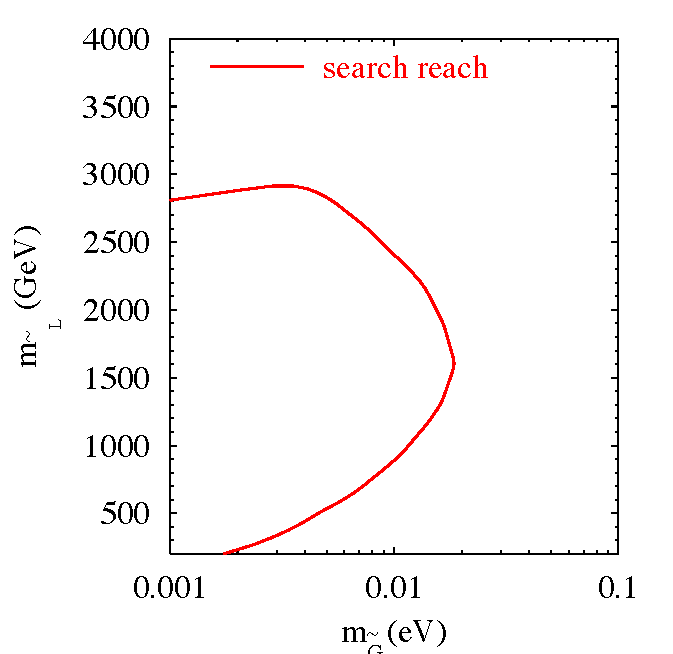
\includegraphics[width=0.5\textwidth]{sample_fig1}
 \caption{Search reach for the $\mu \gamma {\not\!\!E}_{T}$ signal
(as defined in the
   text) for
   300 fb$^{-1}$ integrated luminosity  at the LHC.
}
\label{search}
\end{center}
\end{figure}
We show the region of parameter space corresponding to
\footnote{The
  statistical uncertainties
  on fitted $a$ and $b$ parameters make a negligible difference to the
final numerical results.} $S/\sqrt{B}>5$
and $S\geq10$
for 300 fb$^{-1}$ luminosity option, as a function of smuon mass
and R-parity conserving coupling in Fig.~\ref{search}a.

We now turn to the decay ${\tilde l} \rightarrow {\tilde G} l$. We ignore
sneutrino production in this case because it would lead to an invisible
final state. We have calculated the production matrix element and
the branching ratio and implemented in a parton-level Monte Carlo.
We have used cuts in our analysis on the muon and missing transverse
energy identical
to the $\gamma \mu {\not\!\!E}_{T}$ analysis, i.e.
${\not\!\!E}_{T},E_T^\mu>25$ GeV and $|\eta_\mu|<3$.

\section*{CONCLUSIONS}
Resonant slepton production and its decays into $l \gamma {\tilde G}$ or $l
{\tilde G}$ can be discovered at the LHC for slepton masses into the multi-TeV
region, depending upon the $R_p$ violating coupling and provided that the gravitino is
ultra-light (with a mass less than 0.1 eV). Various $M_T$ distributions will
allow the accurate measurement of sparticle masses involved.


\section*{ACKNOWLEDGEMENTS}
K. Slane would like to thank CERN and LAPTh for hospitality offered
during which some of the work contained herein was performed.

\bibliography{sample_bib}

\end{document}
